%EX TS-program = pdflatex
% !TEX encoding = UTF-8 Unicode

% This is a simple template for a LaTeX document using the "article" class.
% See "book", "report", "letter" for other types of document.

\documentclass[11pt]{article} % use larger type; default would be 10pt
\usepackage[utf8]{inputenc} % set input encoding (not needed with XeLaTeX)

%%% Examples of Article customizations
% These packages are optional, depending whether you want the features they provide.
% See the LaTeX Companion or other references for full information.
\usepackage{amsmath}
\makeatletter
\renewcommand*\env@matrix[1][*\c@MaxMatrixCols c]{%
	\hskip -\arraycolsep
	\let\@ifnextchar\new@ifnextchar
	\array{#1}}
\makeatother

\newcommand{\norm}[1]{\left\lVert#1\right\rVert}
%%% PAGE DIMENSIONS
\usepackage{geometry} % to change the page dimensions
\usepackage{listings}
\usepackage[dvipsnames]{xcolor}
\usepackage{marvosym}
\geometry{a4paper} % or letterpaper (US) or a5paper or....
% \geometry{margin=2in} % for example, change the margins to 2 inches all round
% \geometry{landscape} % set up the page for landscape
%   read geometry.pdf for detailed page layout information

\usepackage{graphicx} % support the \includegraphics command and options
% \usepackage[parfill]{parskip} % Activate to begin paragraphs with an empty line rather than an indent
\usepackage{amssymb}
\usepackage{natbib}
\usepackage{hyperref}
\usepackage{mathrsfs}
%%% PACKAGES
\usepackage{booktabs} % for much better looking tables
\usepackage{array} % for better arrays (eg matrices) in maths
\usepackage{paralist} % very flexible & customisable lists (eg. enumerate/itemize, etc.)
\usepackage{verbatim} % adds environment for commenting out blocks of text & for better verbatim
\usepackage{subfig} % make it possible to include more than one captioned figure/table in a single float
% These packages are all incorporated in the memoir class to one degree or another...
\usepackage{pgfplots}
\usepackage{algorithm}
\usepackage{algpseudocode}
%%% HEADERS & FOOTERS
\usepackage{fancyhdr} % This should be set AFTER setting up the page geometry
\pagestyle{fancy} % options: empty , plain , fancy
\renewcommand{\headrulewidth}{0pt} % customise the layout...
\lhead{}\chead{}\rhead{}
\lfoot{}\cfoot{\thepage}\rfoot{}

%%% SECTION TITLE APPEARANCE
\usepackage{sectsty}
\allsectionsfont{\sffamily\mdseries\upshape} % (See the fntguide.pdf for font help)
% (This matches ConTeXt defaults)
\usepackage[thinc]{esdiff}
\usepackage{bbold}
\usepackage{MnSymbol,wasysym}
%%% ToC (table of contents) APPEARANCE
\usepackage[nottoc,notlof,notlot]{tocbibind} % Put the bibliography in the ToC
\usepackage[titles,subfigure]{tocloft} % Alter the style of the Table of Contents
\renewcommand{\cftsecfont}{\rmfamily\mdseries\upshape}
\renewcommand{\cftsecpagefont}{\rmfamily\mdseries\upshape} % No bold!

%%% END Article customizations

%%% The "real" document content comes below...

\title{Homework 2}
\author{Wei Ye\footnote{2nd year PhD student in Economics Department at Fordham University. Email: wye22@fordham.edu}
    \\ CISC5825 - Computer Algorithm}
\date{Due on Feb 13, 2023}
\begin{document}
\maketitle

\begin{enumerate}[(a)]
    \item The first graph needs 3 colors. $\{color1: v1, v2, v3; color2: v4, v5; color3: v6 \}$. The second graph needs 5 colors. $\{color1: v1, v2;\  color2: v3;\  color3: v4, v5; \ color4: v6, v7;\  color5: v8\}$
    \item For the first graph vertices, see the figure below:
    \begin{figure}[h]
        \includegraphics*[width = 5cm, height = 3cm]{b1.png}
        \centering
    \end{figure}
    Only two colors needed.

    For the second graph vertices, see the figure below:
    \begin{figure}[h]
        \includegraphics*[width = 5cm, height = 3cm]{b2.png}
        \centering
    \end{figure}
    3 colors needed.
    \item 
    \begin{figure}[!htb]
        \begin{minipage}{0.48\textwidth}
          \centering
          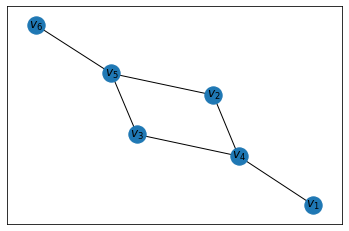
\includegraphics[width=.7\linewidth]{c1.png}
          \caption{First Graph of question c}\label{Fig:Data1}
        \end{minipage}\hfill
        \begin{minipage}{0.48\textwidth}
          \centering
          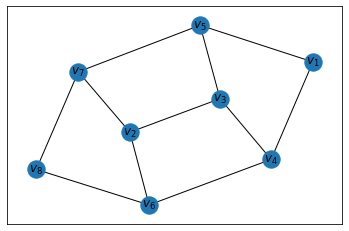
\includegraphics[width=.7\linewidth]{c2.png}
          \caption{second graph of question c}\label{Fig:Data2}
        \end{minipage}
     \end{figure}
 The two figures in the question are fit for this sub-question. For the first graph see \ref{Fig:Data1}, for the second, see \ref{Fig:Data2}
     \item The chromatic number for the first graph is 2. $v_1, v_2, v_3, v_6$ share the same color, $v_4, v_5$ share the same color.
     
     The chromatic number for the second graph is 3. $v_1, v_2$ share the same color, $v_4, v_5, v_8$ share the same color, and $v_3, v_6, v_7$ share the same color.
    
     \item \begin{algorithm}
        \caption{Algorithm for coloring vertices}\label{alg:cap}
        \begin{algorithmic}
        \Procedure {GREEDY}{G, newcolor}
            \State $newcolor \gets \emptyset$
            \For {each uncolored vertex v of G} 
            \If {v is not adjacent to any vertex in newcolor} 
                \State mark v colored
                \State add v to newcolor
            \EndIf
            \EndFor
        \EndProcedure
        \end{algorithmic}
        \end{algorithm}

        \begin{algorithm}
            \caption*{Algorithm for Incompatible Turns}
            \begin{algorithmic}
            \Procedure {GREEDY}{list:T, newcolor}
                \State $newcolor \gets \emptyset$
                \For {each uncolored t of T}
                \If {t does not have common edge to any vertex in newcolors}
                    \State mark t colored
                    \State add t to newcolor
                \EndIf
                \EndFor
            \EndProcedure
            \end{algorithmic}
        \end{algorithm}
\end{enumerate}























\end{document}